\anhang{Experteninterview Ralph B.}\label{anhang:interview-ralph-24.03.2021}
\begin{table}[H]
\begin{tabularx}{\textwidth}{|l|X|}
\hline
    Datum                  & 24.03.2021 \\ \hline
    Thema                  & Initiales Anforderungsinterview \\ \hline
    \begin{tabular}[c]{@{}l@{}}Teilnehmende,\\ Position\end{tabular} & \begin{tabular}[c]{@{}l@{}}Lukas Fruntke, Verfasser\\ Ralph B., Head of Solution - \ac{rnd}\end{tabular}\\ \hline
\end{tabularx}
% \caption{Interviewübersicht Ralph B.}
% \label{tab:interviewuebersicht-ralph-24.03.2021}
\end{table}
\newcommand{\RB}{\textbf{Ralph B.:}~}

\LF Herzlichen Dank Ralph, für deine Bereitschaft zum Interview. Beginnend möchte ich dich fragen, was deine Rolle/Tätigkeiten innerhalb der SPIRIT/21 sind und wie du mit Architekturen zu tun hast.

\RB Meine Rolle in der SPIRIT hat sich schon ien paar mal gewandelt. Aktuell bin ich für den Bereich EBSS Lead \ac{rnd} Verantwortlicher für Forschung und Entwicklung. Als Vorsitzender des Tech- und Architekturboards bin ich für die technologische Qualifizierung von Entwicklungsthemen verantwortlich. Genauso koordiniere ich auch den Einsatz von bestimmten neuen Technologien in den einzelnen Solutions.

\LF Verstehe. Wo siehst du denn Anwendungsgebiete von Referenzarchitekturen in Richtung Zeitreihendatenverarbeitung? 

\RB Welche Architekturen siehst du denn da im Scope? Softwarearchitekturen, oder Infrastrukturachitekturen oder eine andere Architektur?

\LF Ich denke an technische Architekturen, die einen Teil Software und Infrastrukturkomposition umfassen, best practices und eine Art Referenzvorgehen sind \enquote{wie löse ich dieses wiederkehrende Problem, dass immer wieder auftaucht}? Speziell in Richtung Cloud und \ac{AWS} gesehen.

\RB Gut, \ac{AWS} Cloud sehe ich jetzt firmenweit betrachtet nur als ein Teilthema von vielen. Generell zählen für mich da organisatorische und fachliche Richtlinien/Konzepte mit herein. Das geht über die wiederverwendbare technische Lösung hinaus. Vielleicht sollten auch Problem addressiert werden, die momentan nicht akut sind, aber in Zukunft wichtig werden könnten. Generell kann man nicht von einer schlechten Architektur oder einer schlechten Referenzarchitektur sprechen. Klassifizierung in gut oder schlecht ist schwierig. Stattdessen muss man schauen, ob die Architektur auf den Usecase passt oder nicht. 

\LF Konkret Richtung Zeitreihendaten gedacht - wo siehst du konkret die Anwendungsgebiete, wo eine Referenzarchitektur unterstützen könnte?

\RB Das ist generisch immer ein wenig schwierig. Es kommt auf den Anwendungsfall an. Bei Datenerfassung bei \ac{IoT}-Daten muss das Kriterium angelegt werden, ob sehr viele Daten in kurzer Zeit erfasst werden können. Ist die Lösung skalierbar? Wichtig ist aber auch das Ausgeben der Daten: müssen diese instant bereit stehen, oder habe ich da einen Zeitpuffer von fünf Sekunden, bis diese wieder bereit stehen müssen? Wenn ich Daten gespeichert habe, wie lange brauchts die zu lesen? Wo sind Bottlenecks etc.? Im \ac{IoT} Bereich ist speziell der Durchsatz, also die Messages pro Sekunde, die kommen könnten ein Problem, weil jeder Sensor einen Wert sendet, der dann gespeichert werden will. Das hat dann auch mit Verfügbarkeit zu tun - wie bekomme ich die Datenbank dahinter 100\% verfügbar? Die konkreten Anforderungen sind dabei immer unterschiedlich. Wenn man jetzt z.B. \ac{LoRaWAN} Sensordaten hat von 20.000 Sensoren, die alle x Sekunden Daten senden. Kann meine Datenbank diese speichern? Und wenn ich dann einen Report möchte einmal pro Woche, dann möchte ich nicht lange warten, sondern schnell in den Daten navigieren können.

\LF Wir haben ja jetzt schon ein wenig Richtung \ac{IIoT} Daten geschaut. Speziell die Problematik mit den Auswertungen ist da wichtig. Entsprechend dem Datenhalbwertszeitmodell hat es ja drei verschiedene Entscheidertypen, die Daten in unterschiedlicher Zeit benötigen und Entscheidungen treffen. Taktische Entscheider brauchen Daten sehr schnell und trifft auch schnell Entscheidungen. Operative Entscheider brauchen Daten nicht unbedingt nahe Echtzeit und haben einen erweiterten Entscheidungshorizont auf Tage oder Wochen. Strategische Entscheider haben einen wesentlich größeren Entscheidungshorizont gleichzeitig aber auch geringere Anforderungen an die \enquote{Echtzeitigkeit} der Daten. Welche siehst du denn als am wichtigsten an oder für welche würdest du im \ac{IoT} Bereich optimieren?

\RB Ich denke die sind alle gleich wichtig. Im operativen Entscheidungsmodus sollten die Entscheidungsregeln idealerweise automatisiert sein. Einen ausgelösten Feuermelder mit einer Email an einen Verantwortlichen zu koppeln, macht weniger Sinn, als beispielsweise die Werksfeuerwehr zu rufen. Bei unseren bisherigen Projekten ist Latenz nicht so wichtig - da die Geräte bei Bedarf Nachrichten senden oder in Intervallen von 50/60 Sekunden. Latetnz wird aber wieder wichtig, wenn man beispielsweise einen Wassersensor hat, der eine Aktion in der Businesslogik auslöst, die das Wasser bei Kontakt abstellt. Von den historischen Daten kann man ein Dashboard befüllen, wo ein Entscheider einmal die Woche drüberschaut und Entscheidungen trifft. Dann gibt es noch langfristige Usecases - Billing Daten beispielsweise interessieren den Kunden nur einmal im Monat.

\LF Okay, verstehe. Ein bisschen von der Technik weg - es gibt ja Qualitätskriterien zu Referenzarchitekturen - die hatte ich dir schon gesendet. Wie siehst du denn die?

\RB Ich bin da noch eher klassisch. Wenn du jetzt die ISO 9126 anschaust für Qualität von Softwaresystemen (\textit{siehe \autoref{abb:ISO9126}}), hast du noch ein paar andere Kriterien. Was ist denn zufriedenstellende Qualität? Wenn der Kunde zufrieden ist, ist es dann zufriedenstellend? Qualitätsmerkmale sind immer schwammig, weil es nicht \enquote{die Qualität} gibt. Es gibt nur eine passende Architektur, die eine passt besser, die andere schlechter. Qualität ist nicht absolut, sondern relativ anhand von Kriterien. 

\begin{figure}[H]
\centering
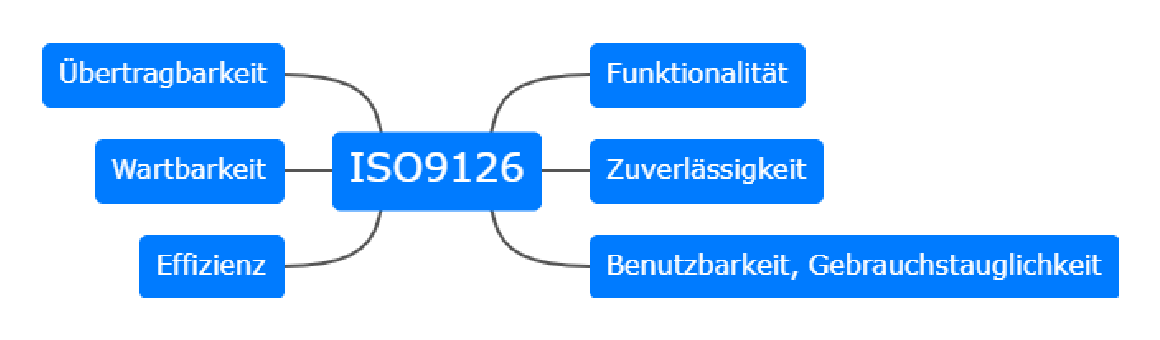
\includegraphics[width=\textwidth]{graphics/ISO-9126.pdf}
\caption[Qualitätskriterien nach ISO 9126]{Qualitätskriterien nach ISO 9126.\footnotemark}
\label{abb:ISO9126}
\end{figure}
\footnotetext{Mit Änderungen entnommen aus: \cite{Johner.2018}}

\LF Ja, für mich gehts darum zu erfahren, welche Kriterien da für den maximierten Nutzen für unsere Zielstakeholder am wichtigsten sind.

\RB Übertragbarkeit zwischen Usecases ist wichtig. Gleichzeitig muss man aber schauen, dass man sich nicht zu sehr fokussiert auf ein Qualitätskriterium. Wenn man beispielsweise bewusst auf single-instance Datenbanken verzichtet und diese immer im Cluster errichtet, erhöht das die Zuverlässigkeit, sprengt aber vielleicht den Preisrahmen des Usecases. 

\LF Da möchte ich mit den Variationspunkten ansetzen, wo ich Entscheidungsoptionen aufzeige wie man die Referenzarchitektur instanziieren kann.

\RB Das Problem ist ja, dass man meistens mit mehr Qualitätskriterien, die man berücksichtigt das Resultat teurer wird.

\LF Da macht das KISS Prinzip dann eher Sinn, oder?

\RB Genau. Der Kunde sollte halt immer den Mehrwert sehen hinter den extra Features die man implementiert. Achte auch auf die Zuverlässigkeit und Modifizierbarkeit.

(0:30)
\TodoW{fertig machen}

